\documentclass[12pt,a4]{article}

\usepackage{graphicx,amsmath,amssymb,amsthm, boxedminipage}



\usepackage{algorithm}
\usepackage{algpseudocode}


\newtheorem{theorem}{Theorem}%[section]
\newtheorem{proposition}[theorem]{Proposition}
\newtheorem{lemma}[theorem]{Lemma}
\newtheorem{corollary}[theorem]{Corollary}
\newtheorem{definition}[theorem]{Definition}



\newcommand{\scalar}[2]{\ensuremath{\langle #1, #2\rangle}}
\newcommand{\floor}[1]{\left\lfloor #1 \right\rfloor}
\newcommand{\ceil}[1]{\left\lceil #1 \right\rceil}
\newcommand{\norm}[1]{\|#1\|}
\newcommand{\pfrac}[2]{\left(\frac{#1}{#2}\right)}
\newcommand{\nth}[1]{#1\textsuperscript{th}}

% \newcommand{\nth}[1]{#1\textsuperscript{th}}
\newcommand{\E}{\mathop{\mathbb{E\/}}}
\newcommand{\N}{\mathbb{N}}

\newcommand{\R}{\mathbb{R}}

\newtheorem{exercise}[theorem]{Exercise}
\newtheorem{exerciseD}[theorem]{*Exercise}
\newtheorem{exerciseDD}[theorem]{**Exercise}

\let\oldexercise\exercise
\renewcommand{\exercise}{\oldexercise\normalfont}

\let\oldexerciseD\exerciseD
\renewcommand{\exerciseD}{\oldexerciseD\normalfont}

\let\oldexerciseDD\exerciseDD
\renewcommand{\exerciseDD}{\oldexerciseDD\normalfont}


 
\begin{document}

\date{}

\title{CS 217 -- Algorithm Design and Analysis \\ 
  \vspace{3mm}
{\large	Shanghai Jiaotong University, Spring 2020\\
}
\author{no code}
}
\maketitle

\setcounter{section}{4}
\section{Flows with Vertex Capacities}


\begin{exercise}
    Let $G = (V,c)$ be a flow network. Prove that flow is ``transitive'' in the following sense: if $r,s,t$ are vertices, 
    and there is an $r$--$s$-flow of value $k$ and an $s$--$t$-flow of value $k$, then there is an $r$--$t$-flow of 
    value $k$.
\end{exercise}
\paragraph{Solution}What we need to do is to show that there exists a path with value k. First of all, if the $r$--$s$-flow and $s$--$t$-flow have no intersection point, we can simply link the two flow and then we get an $r$--$t$-flow of value $k$. But what if the two flow have intersection?
\subparagraph{}If there are some intersections, it's apparently that there will exist some circuits. After eliminating all the circuits, we get a simple path with value k, which is the new $r$--$t$-flow of value $k$.
\subsection{Vertex Disjoint Paths}

Let $G$ be a directed graph. Two paths $p_1, p_2$ from $s$ to $t$ are called {\em vertex disjoint}
if they don't share any vertices except $s$ and $t$. 

\begin{theorem}[Menger's Theorem]
   Let $G$ be a graph and $s \ne t$ two vertices therein. Let $k \in \mathbf{N}_0$. 
   Then exactly one of the following is true:
   \begin{enumerate}
   \item There are $k$ vertex disjoint paths $p_1,\dots,p_k$ from $s$ to $t$; that is, no two $p_i$, $p_j$ share
   any vertex besides $s$ and $t$.
   \item There are vertices $v_1,\dots,v_{k-1} \in V \setminus \{s,t\}$ such that
   $G - \{v_1,\dots, v_{k-1}\}$ contains no $s$--$t$-path.
   \end{enumerate}
\end{theorem}

\begin{exercise}
   Prove Menger's Theorem. You have to prove two things: first, not both cases above can occur (this is rather easy);
   second, one of them must occur (this requires a tool from the lecture).
   
\paragraph{solution}
First we show that not both cases above can occur. In order to show this, we can suppose both 1 and 2 can be true simultaneously. If there are $k$ vertex disjoint paths $p_1,\dots,p_k$ from $s$ to $t$; that is, no two $p_i$, $p_j$ share any vertex besides $s$ and $t$. Because we destroy one s-t path need at least one vertex in this path, and these $k$ paths are vertex disjoint, so we need at least $k$ vertices to destroy all the paths from $s$ to $t$. But 2 says there exits $k-1$ vertices that can destroy all paths in the Graph, which is a contradiction.\\
Next we show that one of them must occur. Suppose 1 not occur, that means there are at most $k-1$ disjoint paths from $S$ to $t$, then we just to prove the max number of disjoint paths equals the least number of vertices which can separate s and t. Construct a directed graph from G, which means replace each edge $xy$ with directed edge $xy$ and $yx$, then we give every vertex with capacity 1 except $s$ and $t$. Then in this case the flow of each edge can only be 0 or 1. According to the max-flow-min-cut theorem, we can easily get there exits a maximum integer flow. Then we can get 
$\text{the max number of disjoint paths} = \text{the max flow} =$the min number of vertices which can separate s and t.
Then we can claim that if 1 not occur, then There are vertices $v_1,\dots,v_{k-1} \in V \setminus \{s,t\}$ such that $G - \{v_1,\dots, v_{k-1}\}$ contains no $s$--$t$-path. Then we prove the Menger's Theorem
   
\end{exercise}






Let $V = \{0,1\}^n$. The $n$-dimensional Hamming cube $H_n$ is the graph $(V,E)$ where
$\{u,v\} \in E$ if $u,v$ differ in exactly one coordinate.
Define the $\nth{i}$ level of $H_n$ as 
\begin{align*}
  L_i := \{u \in V \ | \ \norm{u}_1 = i \} \ ,
\end{align*}
i.e., those vertices $u$ having exactly $i$ coordinates which are $1$.
\begin{center}
  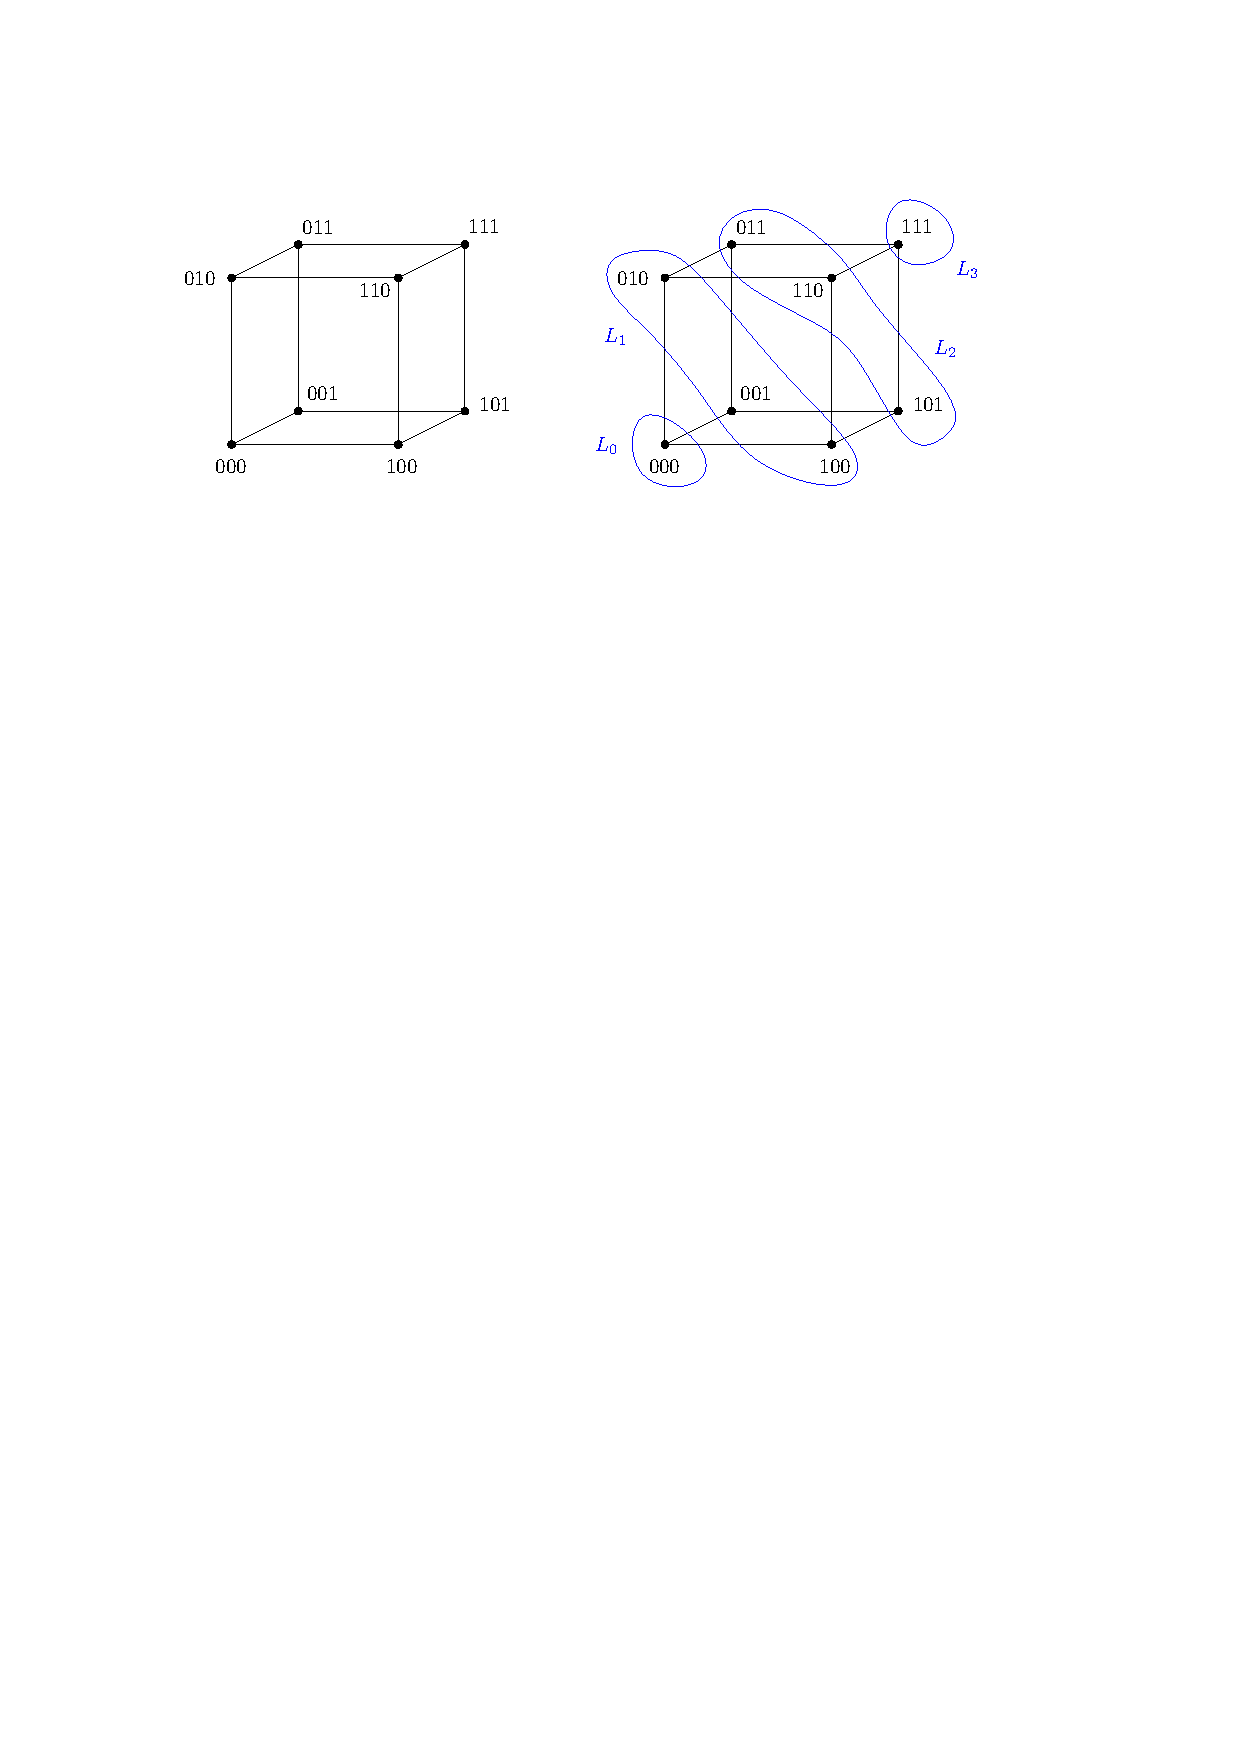
\includegraphics[width=0.8\textwidth]{hamming-3-dim.pdf}\\
  {\small The $3$-dimensional Hamming cube and the four 
    sets $L_0$, $L_1$, $L_2$, $L_3$.}
\end{center}

\begin{exercise}[Matchings in $H_n$]
  Consider the induced bipartite subgraph $H_n[ L_i \cup L_{i+1}]$. This is 
  the graph on vertex set $L_i \cup L_{i+1}$ where two edges are connected
  by an edge if and only if they are connected in $H_n$.
  \medskip

  Show that for $i < n/2$ the graph $H_n[ L_i \cup L_{i+1}]$
  has a matching of size $|L_i| = {n \choose i}$.

\begin{center}
  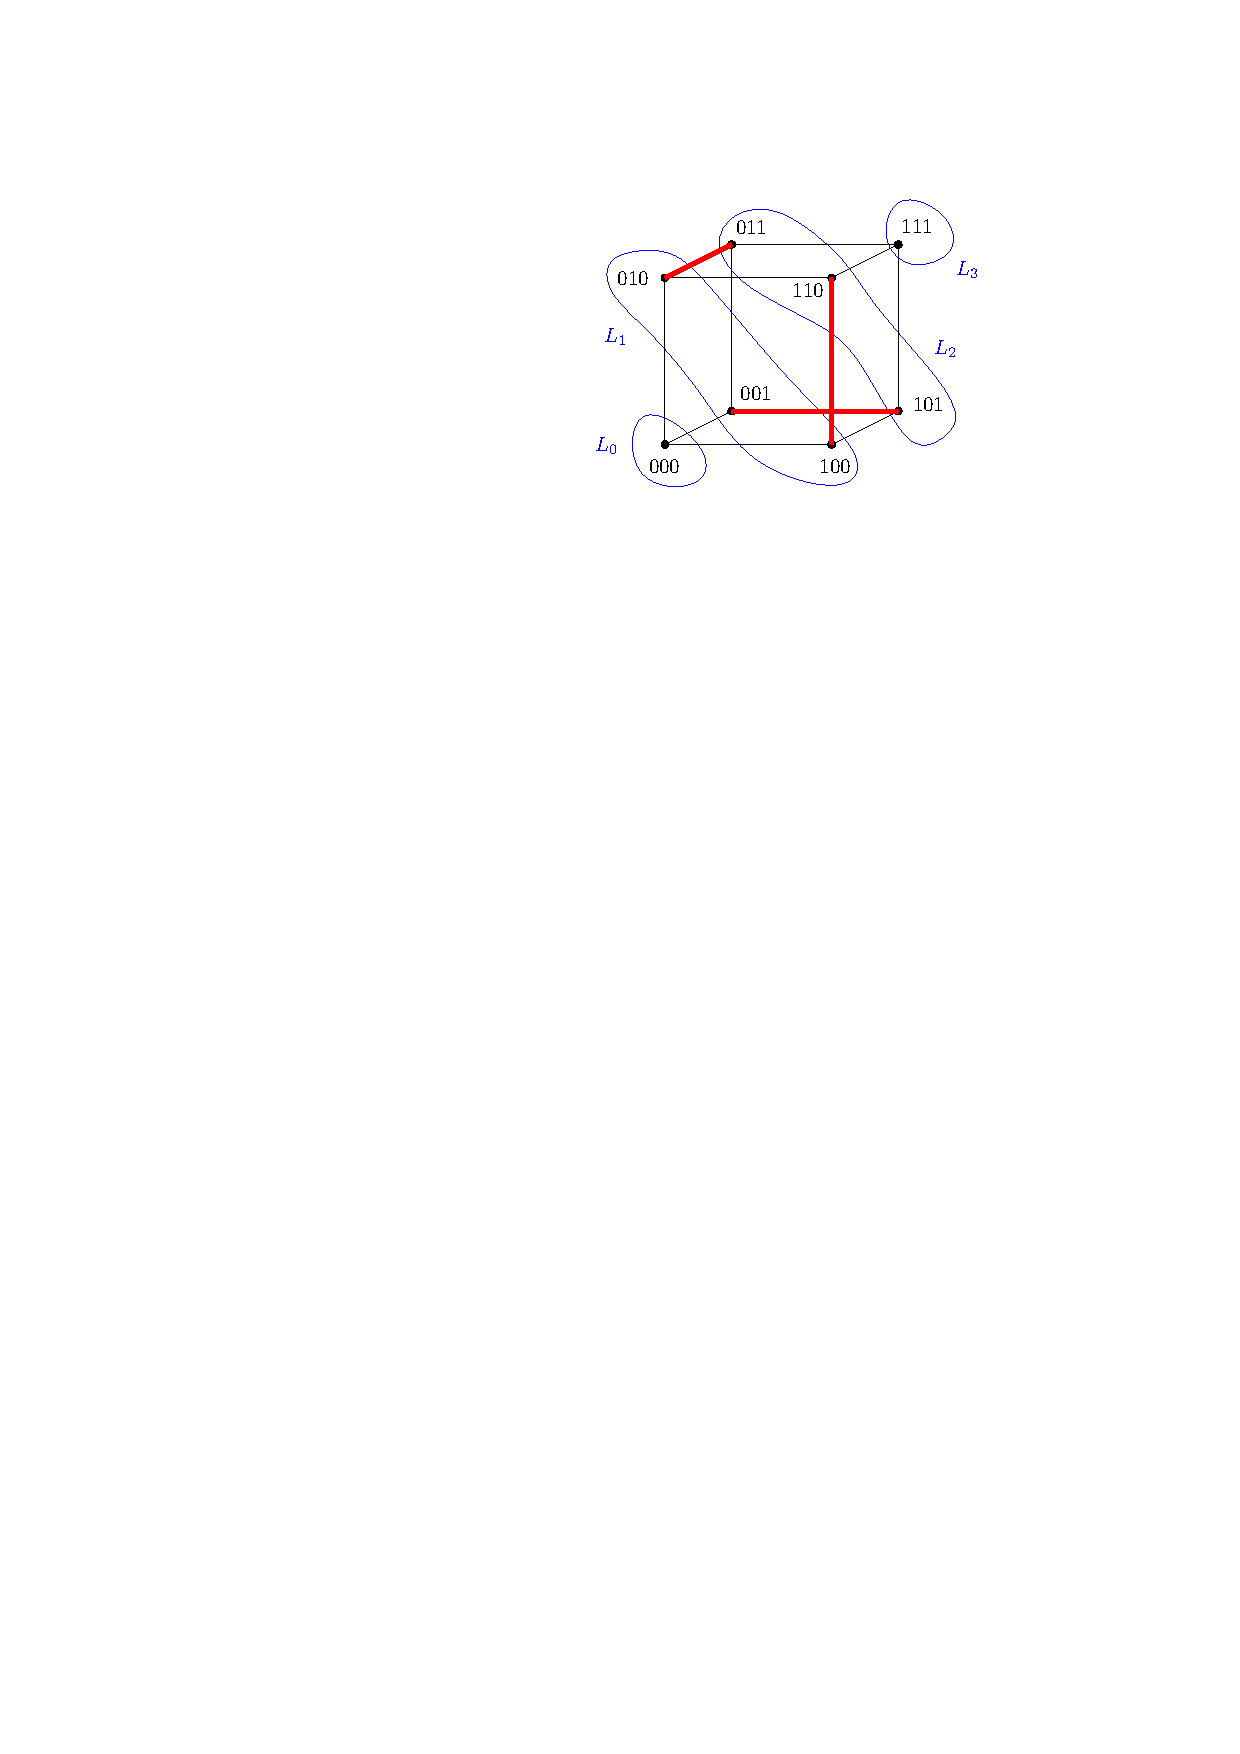
\includegraphics[width=0.4\textwidth]{hamming-3-dim-matching.pdf}\\
  {\small A matching of size $3$ between $L_1$ and $L_2$.}
\end{center}
\label{exercise-matchings-in-H}
\paragraph{Solution}
The graph $H_n[L_i \cup L_{i+1}]$ has a matching of size $|L_i|$ means $H_n[L_i \cup L_{i+1}]$ satisfy Hall condition. 

For any nonempty proper subset $S$ of $L_i$, we know that the degree of vertex in $L_i$ is $n-i$, and the degree of vertex in $L_{i+1}$ is $i+1$. Consider the number of edges between $S$ and $\mathcal{N}(S)$ equals $|S|(n-i)$ or $|\mathcal{N}(S)|(i+1)$.

Hence, $|S|(n-i)=|\mathcal{N}(S)|(i+1)| \land i < n/2 \rightarrow |\mathcal{N}(S)|\geq |S|$. So the graph satisfy Hall condition, 
it has a matching of size $|L_i|$.
\end{exercise}

\begin{exercise} 
  Let $H_n$ be the $n$-dimensional Hamming cube. For $i < n/2$ consider
  $L_i$ and $L_{n-i}$. Note that 
  $|L_i| = {n \choose i} = { n \choose n-i}  = L_{n-i}$, so the 
  $L_i$ and $L_{n-i}$ have the same size.   Show that there are ${n \choose i}$ paths $p_1,p_2,\dots,p_{ {n \choose i}}$
  in $H_n$ such that
  (i) each $p_i$ starts in $L_i$ and ends in $L_{n-i}$;
  (ii) two different paths $p_i,p_j$ do not share any vertices.

  \textbf{Hint 1.} Model this problem as a network flow with vertex capacities. What would 
  the maximum flow be in this network?
  
  \textbf{Hint 2.} It's not {\em that} easy. If you try to work from both sides towards
  the middle by combining matchings between levels, 
  you will certainly run into problems as how to glue things together in the middle.
  I have never seen any ``meet in the middle'' proof that works.
  
  \textbf{Hint 3.} There is a ``direct'' proof by induction that does not require anything
  about network flows.

\paragraph{Solution} .

\texttt{Induction Base} When $n=2$, for $i=0$, it is easy to 
find 2 disjoint paths. 

\texttt{Induction Step} If this statement is always satisfied when $< N$, we can proof it is satisfied when equals $n$.

a) $i=0$. The hyper cube is connected, so exists one path from
$L_0$ to $L_n$.

b) $i > 0$. We need to find $\binom{n}{i}$ disjoint paths from
$L_i$ to $L_{n-i}$, we use $C_{n,i}$ to represent the set of these paths.

Note that $|C_{n,i}|=|C_{n-1,i}|+|C_{n-1,i-1}|$, it tell us can construct $C_{n,i}$ by $C_{n-1,i}$ and $C_{n-1,i-1}$. 

We know the length of each path in $C_{n-1,i-1}$ is $n-2i+2$, and the length of each path in 
$C_{n,i}$ should be $n-2i+1$. Then we construct $|C_{n-1,i-1}|$ paths of $C_{n,i}$. This construction has two steps.

i)  For the kth path $P_k = (v_0^k, v_1^k, \cdots, v_{n-2i+1}^k )$ in $C_{n-1,i-1}$, we insert $P'_k = (v_0^k', v_1^k', \cdots, v_{n-2i}^k')$ to
 $C_{n,i}$, and the $v_j^k' = 2v^k_j + 1$. Obviously, $v_{j}^k'$ has $j + i$ bits,
 and $v_{j}^k', v_{j+1}^k'$ differ in exactly one bit. So $P_k'$ is a valid path.
 
 Note that we discarded the last edge $\{ v_{n-2i}^k,v_{n-2i+1}^k\}$ in $P_k$, let $M = \bigcup_k \{\{v_{n-2i}^k,v_{n-2i+1}^k\}\}$, We can know $M$ is matching between $L_{n-i-1}$ and $L_{n-1}$ of 
 $H_{n-1}$, and its size is $|C_{n-1,i-1}|$. Let us represent the set of paths that we added in first step as
 $A$, 
 
 Then we construct other $|C_{n-1,i}|$ paths.
 
ii) For the kth path $Q_k = (u_0^k, u_1^k, \cdots, u_{n-2i-1}^k )$ in $C_{n-1,i}$, note that its size is only $n-2i$,let $u_j^k' = 2u^k_j$ ,If we want to insert $Q_k' = (u_0^k', u_1^k', \cdots, u_{n-2i-1}^k', u_k)$ to $C_{n,i}$. We need to find the correct $u_k$. If $\exists \{u, v\} \in M$, s.t.$u^k_{n-2i+1}=u$,  let $u_k$ be $2v$, or let $u_k$ be $2u^k_{n-2i+1} + 1$. We can verify that the path is valid. Let us represent the set of paths that we added in the second step as $B$ and $C$,
if $u_k = 2v$, $Q_k' \in B$,  otherwise $Q_k' \in C$. In other words, We distinguish $B$ and $C$ by the last bit of $u_k$. So $|B\cup C| = |C_{n-1,i}|$.

$C_{n,i}=A\cup B\cup C$, then we need to proof for any two paths $P_1, P_2 \in C_{n,i}$, $P_1, P_2$ has 
no common vertex. For the first $n-2i$ vertices in $P_1, P_2$, it satisfy the condition obviously by induction. Let us consider the last vertex. In fact we only need consider $P_1 \in A, P_2 \in C$. Because the last bit of last vertex both are 1, but if $u$ is last vertex of one path in A, then $\lfloor u / 2 \rfloor$ can be find in $M$, otherwise not. 

So $C_{n,i}$ is a valid path set.



 
 


\end{exercise}


\subsection{Matchings and Vertex Covers}

The following exercise was on the final exam of CS 499 (mathematical foundations of computer science) in spring 2019.
\begin{exercise}
    Let $\nu(G)$ denote the size of a maximum matching of $G$. Show that a bipartite graph $G$
    has at most $2^{\nu(G)}$ minimum vertex covers.

\paragraph{Solution}
Consider a maximum matching of bipartite graph $G$, we notice that for two vertices in each edge, one and only one of them will be selected into the minimum vertex covers. Since the size of maximum matching equals to the size of minimum vertex cover, if neither of the vertices is selected, there would be one edge not been covered. Also, if both vertices are selected, this would lead to neither of the vertices is selected in some matching.

Thus, vertices in minimum vertex covers must in all matching of $G$.

Therefore, vertices which can be selected in minimum vertex covers is at most $2^{\nu(G)}$. For each pair pair of vertices, only one of them can be selected, that leads to at most $2^{\nu(G)}$ vertex covers.
    
\end{exercise}


Obviously, this is not  true for general (non-bipartite) graphs: the triangle $K_3$ has $\nu(K_3) = 1$ but it has 
three minimum vertex covers. The five-cycle $C_5$ has $\nu(C_5) = 2$ but has five minimum vertex covers.

\begin{exercise}
   Is there a function $f: \mathbf{N}_0 \rightarrow \mathbf{N}_0$ such that every graph with $\nu(G) = k$ has 
   at most $f(k)$ minimum vertex covers? How small a function $f$ can you obtain?
\end{exercise}

\paragraph{Answer}$f(k)=3^k$
\paragraph{Solution}Let's consider a graph which only containing several cycles. Apparently the cycles of size 3 can reach the upper bound in all the cycles, which is $f(k)=3^k$. Now we want to prove that, after we put a new edge into the graph, the function $f(k)$ won't be larger.
\subparagraph{}First, after putting a new edge into the graph, the value $v(G)=k$ won't decrease, due to the matching in the old graph is also a matching in the new graph. 
\subparagraph{}At the same time, let's consider the problem of minimum vertex covers problem as a kind of 2-sat problem. We need to set all the vertexes with two status, \textsl{selected}(presented as 1) and \textsl{not selected}(presented as 0). Then we have some constrains for edge$(u,v)$, as $status_u|status_v$=1. 
\subparagraph{}After adding an edge, we have more constrains to satisfy and so that, number of minimum vertex covers won't increase.
\subparagraph{}All above shows us that the best scenario is a graph containing several cycles of size 3, which leads to the final answer $f(k)=3^k$.




\end{document}
